To change the number of threads Julia utilizes we use the JULIA\_NUM\_THREADS environment variable.
\begin{minted}[breaklines,escapeinside=||,
                mathescape=true, 
                linenos, 
                numbersep=3pt, 
                gobble=2, 
                frame=lines, 
                fontsize=\small, 
                framesep=2mm]{bash}
    export JULIA_NUM_THREADS=4 # to assign 4 threads to Julia
\end{minted}
\begin{minted}[breaklines,escapeinside=||,
                mathescape=true, 
                linenos, 
                numbersep=3pt, 
                gobble=2, 
                frame=lines, 
                fontsize=\small, 
                framesep=2mm]{julia} 
    # Inside the julia environment type:
    Threads.nthreads() # to check the number of threads julia is using
\end{minted}

Graphs of the results are shown below:
\begin{itemize}
    \item 1 thread
    \begin{figure}[H]
        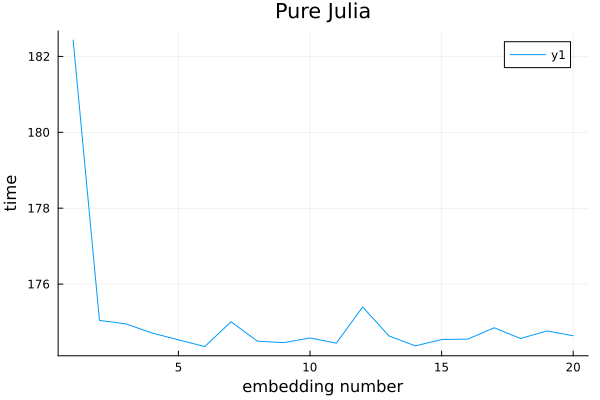
\includegraphics[width=0.5\textwidth]{media/bhembed1.png}
        \caption{Pure Julia (modified) and 1 thread}
    \end{figure}
    \item 2 threads
    \begin{figure}[H]
        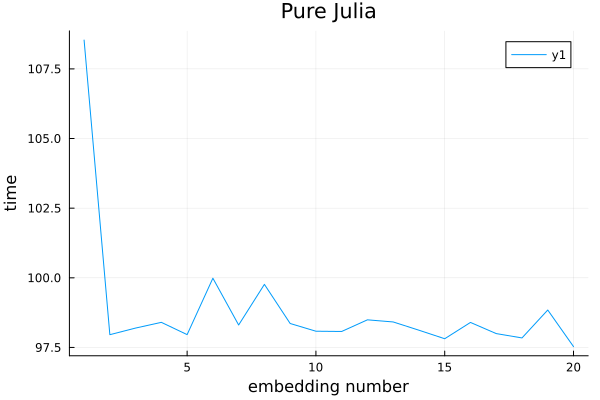
\includegraphics[width=0.5\textwidth]{media/bhembed2.png}
        \caption{Pure Julia (modified) and 2 threads}
    \end{figure}
    \item 4 threads
    \begin{figure}[H]
        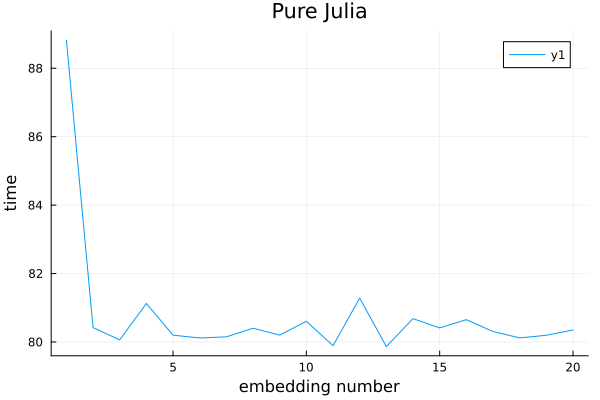
\includegraphics[width=0.5\textwidth]{media/bhembed4.png}
        \caption{Pure Julia (modified) and 4 threads}
    \end{figure}
    \item 8 threads
    \begin{figure}[H]
        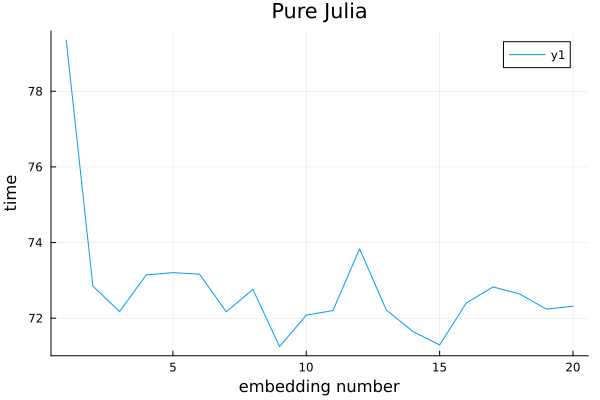
\includegraphics[width=0.5\textwidth]{media/bhembed8.png}
        \caption{Pure Julia (modified) and 8 threads}
    \end{figure}
\end{itemize}